%%%%%%%%%%%%%%%%%%%%%%%%%%%%%%%%%%%%%%%%%%%%%%%
\chapter{Combinatorial Results} \label{chap:comb_res}
%%%%%%%%%%%%%%%%%%%%%%%%%%%%%%%%%%%%%%%%%%%%%%%

In previous studies \cite{Wachter-Zeh:2018}, no general vector solution
outperforming scalar network coding was found for multicast networks
with $h=3$ messages. Hence, we start with a probabilistic argument
to prove that there exists a vector solution outperforming the optimal
linear solution for the $\left(\epsilon=1,\ell=1\right)-\mathcal{N}_{h=3,r,s=4}$
network. Then we generalize the proof to the $\left(\epsilon=1,\ell=1\right)-\mathcal{N}_{h,r,s}$
network.

\section{$\left(\epsilon=1,\ell=1\right)-\mathcal{N}_{h=3,r,s=4}$ Network
\label{sec:Network_e1l1h3rs4}}

\begin{figure}[H]
\caption{The $(\epsilon=1,\ell=1)-\mathcal{N}_{h=3,r,s=4}$ network\label{fig:nw_e1_l1_h3_r_s4}}

\centering{}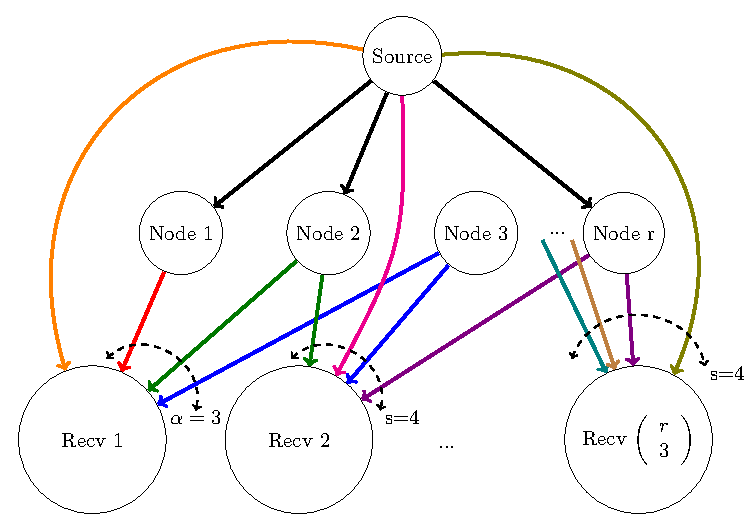
\includegraphics[width=0.5\paperwidth]{E:/Documents/TUM/THESIS/thesisCOD_Ha/figures/nw_e1_l1_h3_r_s4}
\end{figure}

In this subsection, we derive a lower bound on the maximum number
of receivers for the $\left(\epsilon=1,\ell=1\right)-\mathcal{N}_{h=3,r,s=4}$
network. Due to $\alpha=3$, the number of receivers is $N=\left(\begin{array}{c}
r_{vector}\\
3
\end{array}\right)$ by definition in Section \ref{sec:Description_GCN}. To derive the
lower bound, we introduce a rank requirement on incoming packets to
each receiver. 

\begin{figure}[H]
\caption{The vector network coding of $(\epsilon=1,l=1)-\mathcal{N}_{h=3,r,s=4}$
represents as a matrix problem\label{fig:rk_h3}}

\centering{}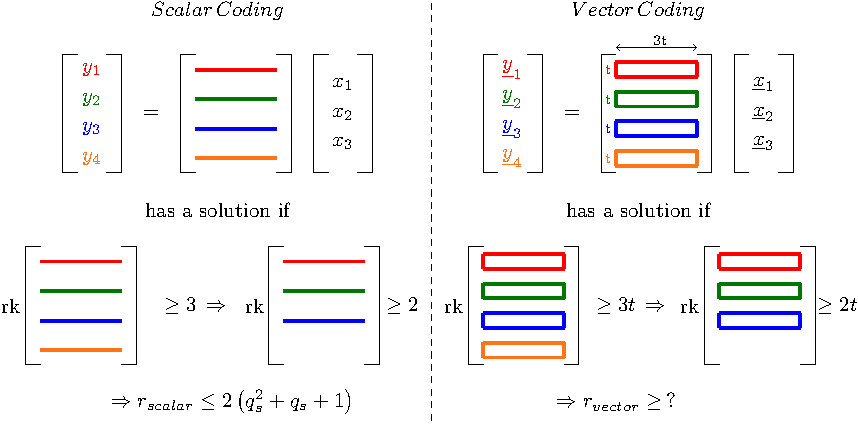
\includegraphics[width=0.6\paperwidth]{E:/Documents/TUM/THESIS/thesisCOD_Ha/figures/rk_h3}
\end{figure}

Following to Equation \ref{eq:linear_system}, each receiver $R_{j}$
must solve a linear equation system of 3 variables with 4 equations
to recover $h=3$ messages as below:

\[
\left[\begin{array}{c}
\boldsymbol{y}_{j}^{\left(r_{1}\right)}\\
\boldsymbol{y}_{j}^{\left(r_{2}\right)}\\
\boldsymbol{y}_{j}^{\left(r_{3}\right)}\\
\boldsymbol{y}_{j}^{\left(r_{4}\right)}
\end{array}\right]=\boldsymbol{A}_{j}\cdot\underline{x}=\left[\begin{array}{c}
\boldsymbol{A}_{j}^{\left(r_{1}\right)}\\
\boldsymbol{A}_{j}^{\left(r_{2}\right)}\\
\boldsymbol{A}_{j}^{\left(r_{3}\right)}\\
\boldsymbol{A}_{j}^{\left(r_{4}\right)}
\end{array}\right]\cdot\left[\begin{array}{c}
\boldsymbol{x}_{1}\\
\boldsymbol{x}_{2}\\
\boldsymbol{x}_{3}
\end{array}\right],
\]

with $\boldsymbol{x}_{i},\boldsymbol{y}_{j}^{\left(v\right)}\in\ensuremath{\mathbb{F}}_{q}^{t},\boldsymbol{A}_{j}^{\left(r_{v}\right)}\in\ensuremath{\mathbb{F}}_{q}^{t\times3t}$
for $v=1,\ldots,4$, and $\boldsymbol{A}_{j}^{\left(r_{1}\right)},\ldots,\boldsymbol{A}_{j}^{\left(r_{3}\right)}$
must be distinct.

The network is solvable, if $\boldsymbol{A}_{j}$ has full-rank, i.e.
$\boldsymbol{A}_{j_{v}}$ must satisfy:

\[
rk\left[\begin{array}{c}
\boldsymbol{A}_{j}^{\left(r_{1}\right)}\\
\boldsymbol{A}_{j}^{\left(r_{2}\right)}\\
\boldsymbol{A}_{j}^{\left(r_{3}\right)}\\
\boldsymbol{A}_{j}^{\left(r_{4}\right)}
\end{array}\right]\geq3t
\]

Because coding coefficients for $\boldsymbol{A}_{j}^{\left(r_{4}\right)}$
can be independently chosen for any receiver $R_{j}$, there always
exists $\boldsymbol{A}_{j}^{\left(r_{4}\right)}$ such that,

\begin{equation}
rk\left[\begin{array}{c}
\boldsymbol{A}_{j}^{\left(r_{1}\right)}\\
\boldsymbol{A}_{j}^{\left(r_{2}\right)}\\
\boldsymbol{A}_{j}^{\left(r_{3}\right)}
\end{array}\right]\geq2t\label{eq:rk_rqm_e1l1h3s4}
\end{equation}

if and only if $rk\left[\boldsymbol{A}_{j}\right]\geq3t$.

By this constraint, the problem is thus described as below:

\[
\underset{rk\left[\boldsymbol{A}_{j}\right]\geq3t}{min}\,r_{vector}
\]

$\boldsymbol{A}_{j}^{\left(r_{1}\right)},\boldsymbol{A}_{j}^{\left(r_{2}\right)},\boldsymbol{A}_{j}^{\left(r_{3}\right)}$
are matrices formed on any 3 of $r$ links from nodes to receivers,
i.e. these 3 matrices are randomly chosen from a set of $r$ matrices.
We formalize the problem by an approach with Lov\'asz local lemma,
which was initially proposed by Schwartz in \cite{MosheSchwartz:2018}.
\begin{lem}[Symmetric Lov\'asz local lemma (LLL) \cite{Schwarz:2013}]
 A set of events $\mathcal{E}_{i}$, with $i=1,\ldots,n$, such that
each event occurs with probability at most $p$. If each event is
independent of all others except for at most $d$ of them and $4dp\leq1$,
then: $Pr\left[\stackrel[i=1]{n}{\bigcap}\overline{\mathcal{E}}_{i}\right]>0$.
\label{thm:LLL}
\end{lem}
%
\begin{lem}
$p\leq\Theta\left(q^{-t^{2}-2t-1}\right),\forall t\geq2$. \label{lem:prob_p_LLL_formula}
\end{lem}
\begin{proof}
In Lemma \ref{thm:LLL}, each event $\mathcal{E}_{i}$ is a \textit{bad
event}, whose occurrence is undesirable. Following to Equation \ref{eq:rk_rqm_e1l1h3s4},
such a event occurs when $rk\left[\boldsymbol{A}_{j}\right]<3t$,
and its probability is bounded by $p$ (with $0\leq p\leq1$) as following,

\begin{equation}
Pr\left[\mathcal{E}_{i}\right]=Pr\left[rk\left[\begin{array}{c}
\boldsymbol{A}_{j}^{\left(r_{1}\right)}\\
\boldsymbol{A}_{j}^{\left(r_{1}\right)}\\
\boldsymbol{A}_{j}^{\left(r_{3}\right)}
\end{array}\right]<2t\right]\leq p.\label{eq:p_in_LLL}
\end{equation}

Regarding to the left-hand side,

\begin{eqnarray}
Pr\left[rk\left[\begin{array}{c}
\boldsymbol{A}_{j}^{\left(r_{1}\right)}\\
\boldsymbol{A}_{j}^{\left(r_{2}\right)}\\
\boldsymbol{A}_{j}^{\left(r_{3}\right)}
\end{array}\right]<2t\right] & = & \stackrel[i=0]{2t-1}{\mathop{\sum}}Pr\left[rk\left[\begin{array}{c}
\boldsymbol{A}_{j}^{\left(r_{1}\right)}\\
\boldsymbol{A}_{j}^{\left(r_{2}\right)}\\
\boldsymbol{A}_{j}^{\left(r_{3}\right)}
\end{array}\right]=i\right]\nonumber \\
 & \overset{1}{=} & \stackrel[i=0]{2t-1}{\mathop{\sum}}\frac{N_{i,m,n}}{q^{m\cdot n}}\nonumber \\
 & = & \stackrel[i=0]{2t-1}{\mathop{\sum}}\frac{\stackrel[j=0]{i-1}{\mathop{\prod}}\frac{\left(q^{m}-q^{j}\right)\left(q^{n}-q^{j}\right)}{q^{i}-q^{j}}}{q^{m\cdot n}}\nonumber \\
 & \overset{2}{=} & \stackrel[i=0]{2t-1}{\mathop{\sum}}\frac{\stackrel[j=0]{i-1}{\mathop{\prod}}\frac{\left(q^{3t}-q^{j}\right)^{2}}{q^{i}-q^{j}}}{q^{9t^{2}}}.\label{eq:p_eq_h3}
\end{eqnarray}

(1): The formula for the umber of $\left[m\times n\right]$ matrices
of rank $i$ over $\ensuremath{\mathbb{F}}_{q}$ was proved in \cite{Overbeck:2007}.

(2): $\boldsymbol{A}_{j}^{\left(r_{1}\right)},\boldsymbol{A}_{j}^{\left(r_{2}\right)},\boldsymbol{A}_{j}^{\left(r_{3}\right)}$
vertically together form a $\left[3t\times3t\right]$ matrix.

We consider the numerator of Equation (\ref{eq:p_eq_h3}): $\stackrel[j=0]{i-1}{\mathop{\prod}}\frac{\left(q^{3t}-q^{j}\right)^{2}}{q^{i}-q^{j}}=\frac{p_{N}^{(i)}(q)}{p_{D}^{(i)}(q)}=p^{(i)}(q)$.

Due to $i$-times product and large $t$: $\left.\begin{array}{c}
deg\left(p_{N}^{(i)}(q)\right)=q^{i6t}\\
deg\left(p_{D}^{(i)}(q)\right)=q^{i^{2}}
\end{array}\right\} \Rightarrow p^{(i)}(q)\approx q^{i6t-i^{2}}$.

Therefore, we have: $\stackrel[i=0]{2t-1}{\mathop{\sum}}\stackrel[j=0]{i-1}{\mathop{\prod}}\frac{\left(q^{3t}-q^{j}\right)^{2}}{q^{i}-q^{j}}=\stackrel[i=0]{2t-1}{\mathop{\sum}}p^{(i)}(q)\approx\stackrel[i=0]{2t-1}{\mathop{\sum}}q^{i6t-i^{2}}$.

To maximize the sum, we set derivation of it to 0 and find the corresponding
root: 

\begin{eqnarray*}
 & \left(i6t-i^{2}\right)^{'} & =0\\
\Leftrightarrow & 6t-2i & =0\\
\Leftrightarrow & i & =3t
\end{eqnarray*}

However, the upper limit of the sum is $\left(2t-1\right)$, which
is less than $3t$ for all $t\geq2$.

\[
\Rightarrow max\left\{ q^{i6t-i^{2}}:i=0,2\ldots,2t-1\right\} =\left.q^{i6t-i^{2}}\right|_{i=2t-1}=q^{8t^{2}-2t-1}
\]

Hence, by using the exact bound $\Theta$, we have:

\[
\underset{i}{max}\left[\stackrel[i=0]{2t-1}{\mathop{\sum}}p^{(i)}(q)\right]\in\Theta\left(max\left\{ q^{i6t-i^{2}}:i=1,2\ldots,2t-1\right\} \right)=\Theta\left(q^{8t^{2}-2t-1}\right)
\]

\[
\Rightarrow\underset{i}{max}\left[\frac{\stackrel[i=0]{2t-1}{\mathop{\sum}}p^{(i)}(q)}{q^{9t^{2}}}\right]\in\Theta\left(q^{-t^{2}-2t-1}\right)
\]

\[
\Rightarrow p\leq\Theta\left(q^{-t^{2}-2t-1}\right)
\]
\end{proof}
\begin{lem}
$d\leq\frac{3}{2}r^{2}$. \label{lem:dependecy_d_LLL}
\end{lem}
\begin{proof}
Because $d$ is a function of $r$ in our problem, we denote $d$
in Lemma \ref{thm:LLL} specifically by $d(r)$. The Local lemma \ref{thm:LLL}
allows dependence among at most $d(r)$ events, i.e. each event considered
under the Local lemma must no be independent to each other.

Furthermore, $\boldsymbol{A}_{j}^{\left(r_{1}\right)},\boldsymbol{A}_{j}^{\left(r_{2}\right)},\boldsymbol{A}_{j}^{\left(r_{3}\right)}$
are matrices formed on any 3 of $r$ links from nodes to receivers.
Assume that 1 of $r$ links is firstly chosen to form the matrix $\boldsymbol{A}_{j}^{\left(r_{1}\right)}$,
then there are $\left(\begin{array}{c}
r-1\\
2
\end{array}\right)$ posibilities left to choose $\boldsymbol{A}_{j}^{\left(r_{2}\right)}$
and $\boldsymbol{A}_{j}^{\left(r_{3}\right)}$ from $r-1$ links.
However, such a link can also be chosen firstly to form $\boldsymbol{A}_{j}^{\left(r_{2}\right)}$
or $\boldsymbol{A}_{j}^{\left(r_{3}\right)}$ instead. Therefore,
we have a upper bound for $d(r)$ as following,

\[
d(r)\leq3\cdot\left(\begin{array}{c}
r-1\\
2
\end{array}\right)=3\cdot\frac{\left(r-1\right)\left(r-2\right)}{2}=\frac{3}{2}\left(r^{2}-3r+2\right)
\]

\[
\Rightarrow d(r)\leq\frac{3}{2}r^{2}
\]
\end{proof}
Example:

$r\in\left\{ 1,2,3,4\right\} $. Our sample space to draw any 3 matrices
with orders has in total $\left(\begin{array}{c}
4\\
3
\end{array}\right)=4$ samples.

Assume the link 1 is firstly chosen to form the matrix $\boldsymbol{A}_{j}^{\left(r_{1}\right)}$,
we have $\left(\begin{array}{c}
3\\
2
\end{array}\right)=3$ possibilities: $\left[\begin{array}{c}
1\\
2\\
3
\end{array}\right],\left[\begin{array}{c}
1\\
2\\
4
\end{array}\right]$ and $\left[\begin{array}{c}
1\\
3\\
4
\end{array}\right]$. The existence of $1$ in $\left[\begin{array}{c}
1\\
2\\
3
\end{array}\right]$ gives us some information on $rk\left[\begin{array}{c}
1\\
2\\
4
\end{array}\right]$ or $rk\left[\begin{array}{c}
1\\
3\\
4
\end{array}\right]$, which means these events $rk\left[\begin{array}{c}
\boldsymbol{A}_{j}^{\left(r_{1}\right)}\\
\boldsymbol{A}_{j}^{\left(r_{1}\right)}\\
\boldsymbol{A}_{j}^{\left(r_{3}\right)}
\end{array}\right]<2t$ are dependent. 

We also have 3 posibilities, when we choose the link 1 to form the
matrix $\boldsymbol{A}_{j}^{\left(r_{2}\right)}$: $\left[\begin{array}{c}
2\\
1\\
3
\end{array}\right],\left[\begin{array}{c}
2\\
1\\
4
\end{array}\right]$ and $\left[\begin{array}{c}
3\\
1\\
4
\end{array}\right]$. 

There are again 3 posibilities, when we choose the link $1$ to form
the matrix $\boldsymbol{A}_{j}^{\left(r_{3}\right)}$: $\left[\begin{array}{c}
2\\
3\\
1
\end{array}\right],\left[\begin{array}{c}
2\\
4\\
1
\end{array}\right]$ and $\left[\begin{array}{c}
3\\
4\\
1
\end{array}\right]$.

Let's denote the event $rk\left[\begin{array}{c}
1\\
2\\
3
\end{array}\right]<2t$ by $\mathcal{E}_{1}$. It is clearly to see that $Pr\left[\begin{array}{c|c}
rk\left[\begin{array}{c}
2\\
1\\
3
\end{array}\right]<2t & \mathcal{E}_{1}\end{array}\right]=1$. The bound in Lemma \ref{lem:dependecy_d_LLL} is a bit loose, because
we do not neglect unsuitable matrices, e.g. $\left[\begin{array}{c}
3\\
1\\
4
\end{array}\right]$. In the other words, there exists at most 9 events are dependent. 

>\textcompwordmark >\textcompwordmark > IS THIS EXAMPLE CONVINCING
ENOUGH? WHY IS IT NOT $d(r)\leq3\cdot r\cdot\left(\begin{array}{c}
r-1\\
2
\end{array}\right)=$?
\begin{thm}
If $r\leq\Omega\left(q^{t^{2}/2+\mathcal{O}\left(t\right)}\right)$,
then there exists a vector solution for the $\left(\epsilon=1,l=1\right)-\mathcal{N}_{h=3,r,s=4}$
network. \label{theo:r_for_vector_sol_e1l1h3rs4}
\end{thm}
\begin{proof}
The Local lemma \ref{thm:LLL} shows that there is a positive probability
that none of bad events occurs: $Pr\left[\stackrel[i=1]{n}{\bigcap}\overline{\mathcal{E}}_{i}\right]>0$.

By the intersection rule, none of bad events is equivalent to an event
$T$ that its set of outcomes are all desirable, i.e. these outcomes
satisfy the Equation \ref{eq:rk_rqm_e1l1h3s4}:

\[
T=\stackrel[i=1]{n}{\bigcap}\overline{\mathcal{E}}_{i}=rk\left[\begin{array}{c}
\boldsymbol{A}_{j}^{\left(r_{1}\right)}\\
\boldsymbol{A}_{j}^{\left(r_{2}\right)}\\
\boldsymbol{A}_{j}^{\left(r_{3}\right)}
\end{array}\right]\geq2t,\forall1\leq r_{1}<r_{2}<r_{3}\leq r.
\]

The probability of event $T$ indicates a measure quantifying the
likelihood that we are able to construct $rk\left[\boldsymbol{A}_{j}\right]\geq3t$
given $r$ links. It means that a vector solution exists if and only
if the Local lemma \ref{thm:LLL} is satisfied such that: $4\cdot p\cdot d(r)\leq1,\forall r\leq r_{max,vector}$.
Therefore, we must find a lower bound of $r_{max,vector}$. Furthermore,
we have $d\leq\frac{3}{2}r^{2}$ following to Lemma \ref{lem:dependecy_d_LLL},
which gives: $4\cdot p\cdot\frac{3}{2}r^{2}\leq1\Rightarrow r\leq\sqrt{\frac{1}{6p}}=r_{max,vector}$.
Thus, finding $min\left[r_{max,vector}\right]$ is equivalent to maximize
$p$. 

By Lemma \ref{lem:prob_p_LLL_formula}, we have $p\leq\Theta\left(q^{-t^{2}-2t-1}\right)$,

\[
\Rightarrow min\left[r_{max,vector}\right]\in\Omega\left(\sqrt{\frac{1}{6p}}\right)=\Omega\left(\sqrt{\frac{1}{6q^{-t^{2}-2t-1}}}\right)=\Omega\left(q^{t^{2}/2+\mathcal{O}\left(t\right)}\right).
\]

Hence, the Local lemma in \ref{thm:LLL} is satisfied, when $r\leq\Omega\left(q^{t^{2}/2+\mathcal{O}\left(t\right)}\right)$.
None of bad events occurs, so there exists a vector solution for such
$r$.
\end{proof}
\begin{cor}
The $\left(\epsilon=1,\ell=1\right)-\mathcal{N}_{h=3,r,s=4}$ network
has a vector solution with a gap $q^{t^{2}/4+\mathcal{O}(t)}$.
\end{cor}
In \cite[Sec. VIII-C]{Wachter-Zeh:2018}, we have that $r_{max,scalar}\in\mathcal{O}\left(q_{\mathrm{s}}^{2}\right)$,
where they proved that 

\begin{equation}
r_{scalar}\leq2\left[\begin{array}{c}
3\\
1
\end{array}\right]_{q_{s}}=2\left(q_{s}^{2}+q_{s}+1\right).\label{eq:r_scalar_max}
\end{equation}
 

Following to Section \ref{subsec:Comparison-between-scalar-and-vector-sol}
and Theorem \ref{theo:r_for_vector_sol_e1l1h3rs4}, we have the gap
size 

\begin{eqnarray}
 & r_{max,scalar} & =min\left[r_{max,vector}\right]\nonumber \\
\Leftrightarrow & q_{\mathrm{s}}^{2} & =q^{t^{2}/2+\mathcal{O}(t)}\nonumber \\
\Leftrightarrow & q_{\mathrm{s}} & ^{=}q^{t^{2}/4+\mathcal{O}(t)}\nonumber \\
\Rightarrow & g & =q_{\mathrm{s}}-q_{v}=q^{t^{2}/4+\mathcal{O}(t)}\label{eq:gap_e1l1h3rs4}
\end{eqnarray}

By varying $t$ in Equation (\ref{eq:p_eq_h3}), we have the following
table:

\begin{table}[H]
\caption{$r$ over variations of t\label{tab:r_over_t}}

\begin{centering}
\begin{tabular}{|c|c|c|}
\hline 
t & Scalar Solution & Vector Solution\tabularnewline
\hline 
\hline 
1 & $r_{scalar}\leq14$ & $r_{vector}\geq3$\tabularnewline
\hline 
2 & $r_{scalar}\leq42$ & $r_{vector}\geq7\,\left(67^{*},\,89^{**}\right)$\tabularnewline
\hline 
3 & $r_{scalar}\leq146$ & $r_{vector}\geq62\,\left(166^{*}\right)$ \tabularnewline
\hline 
4 & $r_{scalar}\leq546$ & $r_{vector}\geq1317$\tabularnewline
\hline 
5 & $r_{scalar}\leq2114$ & $r_{vector}\geq58472$\tabularnewline
\hline 
6 & $r_{scalar}\leq8322$ & $r_{vector}>10^{6}$\tabularnewline
\hline 
\end{tabular}
\par\end{centering}
{*}, {*}{*}: computational results in construction 1 and construction
2 respectively
\end{table}

In the table (\ref{tab:r_over_t}), the vector solution outperforms
the scalar solution when $t\geq4$ for the network $\left(\epsilon=1,\ell=1\right)-\ensuremath{N}_{h=3,r,s=4}$.
This is sufficient, we show in Section 6 computational results which
vector solutions outperform scalar solutions in case of $t=2$ and
$t=3$.

\section{$\left(\epsilon=1,\ell=1\right)-\mathcal{N}_{h,r,s}$ Network \label{sec:e1l1_nw}}

\subsection{Find the lower bound of $r_{max,vector}$}

As previous, $\boldsymbol{A}_{j}^{\left(r_{1}\right)},\ldots,\boldsymbol{A}_{j}^{\left(r_{h-\epsilon}\right)}\in\ensuremath{\mathbb{F}}_{q}^{t\times ht}$
and we need to satisfy the following:

\[
rk\left[\begin{array}{c}
\boldsymbol{A}_{j}^{\left(r_{1}\right)}\\
\vdots\\
\boldsymbol{A}_{j}^{\left(r_{h-\epsilon}\right)}
\end{array}\right]\geq ht-t\Leftrightarrow rk\left[\boldsymbol{A}_{j}\right]\geq(h-1)t
\]

We can formulate it by the following coding problem in Grassmannian:

\noindent\fbox{\begin{minipage}[t]{1\columnwidth - 2\fboxsep - 2\fboxrule}%
Find the largest set of subspaces from $\mathcal{G}_{q}\left(ht,t\right)$
such that any $\alpha$ subspaces of the set span a subspace of dimension
at least $\left(h-1\right)t$.%
\end{minipage}}

Similar with $\left(\epsilon=1,\ell=1\right)-\ensuremath{N}_{3,r,4}$,
we consider $p$ to proceed the Local lemma \ref{thm:LLL}:

\begin{equation}
Pr\left[rk\left[\boldsymbol{A}_{j}\right]<(h-1)t\right]\leq p\label{eq:p_e1l1}
\end{equation}

\begin{lem}
$p\leq\Theta\left(q^{\left(h-\alpha\right)t^{2}+\mathcal{O}(t)}\right),\forall t\geq2$.
\end{lem}
\begin{proof}
Regarding to the left-hand side in Equation \ref{eq:p_e1l1}:

\begin{eqnarray}
Pr\left[rk\left[\boldsymbol{A}_{j}\right]<(h-1)t\right] & = & \stackrel[i=0]{(h-1)t-1}{\mathop{\sum}}Pr\left[rk\left[\boldsymbol{A}\right]=i\right]\nonumber \\
 & \overset{1}{=} & \stackrel[i=0]{(h-1)t-1}{\mathop{\sum}}\frac{N_{i,\alpha t,ht}}{q^{\left(\alpha t\right)\left(ht\right)}}\nonumber \\
 & = & \frac{1}{q^{\left(\alpha h\right)t^{2}}}\cdot\stackrel[i=0]{(h-1)t-1}{\mathop{\sum}}\stackrel[j=0]{i-1}{\mathop{\prod}}\frac{\left(q^{\alpha t}-q^{j}\right)\left(q^{ht}-q^{j}\right)}{q^{i}-q^{j}}.\label{eq:general_nw_calc_p}
\end{eqnarray}

(1): The formula for the umber of $\left[m\times n\right]$ matrices
of rank $i$ over $\ensuremath{\mathbb{F}}_{q}$ was proved in \cite{Overbeck:2007}.

We consider firstly the product$\stackrel[j=0]{i-1}{\mathop{\prod}}\frac{\left(q^{\alpha t}-q^{j}\right)\left(q^{ht}-q^{j}\right)}{q^{i}-q^{j}}=\frac{p_{N}^{(i)}(q)}{p_{D}^{(i)}(q)}=p^{(i)}(q)$.

For $t\rightarrow\infty$: $\left.\begin{array}{c}
deg\left(p_{N}^{(i)}(q)\right)=q^{i(\alpha t+ht)}\\
deg\left(p_{D}^{(i)}(q)\right)=q^{i^{2}}
\end{array}\right\} \Rightarrow p^{(i)}(q)\approx q^{i(\alpha t+ht)-i^{2}}.$

Now, we evaluate $f(i)=i(\alpha t+ht)-i^{2}$ to find its maximum
point by its derivation : 

$\dot{f}(i^{*})=0\Leftrightarrow(\alpha t+ht)-2i^{*}=0\Leftrightarrow i^{*}=\frac{\alpha t+ht}{2}$

We then check whether this point within the range $i=0,\ldots,(h-1)t-1$
as following: $0\leq\frac{\alpha t+ht}{2}\leq(h-1)t-1$.

With regards to the lower bound: $0\leq\frac{\alpha t+ht}{2}\Leftrightarrow t\geq\frac{2}{\alpha+h}$,
which is always true due to the given $t\geq2$ and $\alpha,h\geq3$.

Regarding to the upper bound: $\frac{\alpha t+ht}{2}\leq(h-1)t-1\Leftrightarrow t\leq\frac{-2}{\alpha+2-h}$
with $\alpha+2>h$ due to the given $\alpha l+\epsilon=\alpha+1\geq h$.
This cannot happen because of $t\geq2$, i.e. this maximum point is
over then upper-range limit.

\begin{eqnarray*}
\Rightarrow & max\left\{ q^{i(\alpha t+ht)-i^{2}}:i=1,\ldots,(h-1)t-1\right\}  & =\left.q^{i(\alpha t+ht)-i^{2}}\right|_{i=(h-1)t-1}\\
 &  & =q^{\left[\left(h-1\right)\left(\alpha+1\right)\right]t^{2}-\left(\alpha-h+2\right)t-1}.
\end{eqnarray*}

Secondly, we apply the maximum value with the sum, we have:

\begin{eqnarray*}
 & max\left[\stackrel[i=0]{(h-1)t-1}{\mathop{\sum}}p^{(i)}(q)\right] & \in\Theta\left(q^{\left[\left(h-1\right)\left(\alpha+1\right)\right]t^{2}+\mathcal{O}(t)}\right)\\
\Rightarrow & max\left[\frac{\stackrel[i=0]{(h-1)t-1}{\mathop{\sum}}p^{(i)}(q)}{q^{\left(\alpha h\right)t^{2}}}\right] & \in\left(\frac{q^{\left[\left(h-1\right)\left(\alpha+1\right)\right]t^{2}+\mathcal{O}(t)}}{q^{\left(\alpha h\right)t^{2}}}\right)
\end{eqnarray*}

\[
\Rightarrow p\leq\Theta\left(q^{\left(h-\alpha\right)t^{2}+\mathcal{O}(t)}\right)
\]
\end{proof}
\begin{lem}
$d\leq\frac{\alpha}{\left(\alpha-1\right)!}r^{^{\alpha-1}}$\label{lem:d_e1l1}.
\end{lem}
\begin{proof}
Similar with $\left(\epsilon=1,\ell=1\right)-\ensuremath{N}_{3,r,4}$,
we have:

\[
d\leq\alpha\left(\begin{array}{c}
r-1\\
\alpha-1
\end{array}\right)=\alpha\frac{\left(r-1\right)\ldots\left(r-\alpha+1\right)}{\left(\alpha-1\right)!}\leq\frac{\alpha}{\left(\alpha-1\right)!}r^{^{\alpha-1}}
\]
\end{proof}
\begin{thm}
If $r\leq\Omega\left(q^{\frac{h-\alpha-1}{1-\alpha}t^{2}+\mathcal{O}(t)}\right)$,
then there exists a vector solution for the $\left(\epsilon=1,\ell=1\right)-\ensuremath{N}_{h,r,s}$
network.
\end{thm}
\begin{proof}
As previous, satisfying LLL \ref{thm:LLL} is equivalent to an existence
of a vector solution. We need $4dp\leq1$, and following to Lemma
\ref{lem:d_e1l1}: $d\leq\frac{\alpha}{\left(\alpha-1\right)!}r^{^{\alpha-1}}\Rightarrow r\leq\left(\frac{\left(\alpha-1\right)!}{4\alpha}\cdot\frac{1}{p}\right)^{\frac{1}{\alpha-1}}=r_{max,vector}$.
We thus again find a lower bound of $r_{max,vector}$.

By Lemma \ref{lem:d_e1l1}, we have $p\leq\Theta\left(q^{\left(h-\alpha\right)t^{2}+\mathcal{O}(t)}\right),\forall t\geq2$,

$\Rightarrow min\left[r_{max,vector}\right]\in\Omega\left(q^{\frac{h-\alpha-1}{1-\alpha}t^{2}+\mathcal{O}(t)}\right)$.

Hence, the Local lemma \ref{thm:LLL} is satisfied, when $r\leq\Omega\left(q^{\frac{h-\alpha-1}{1-\alpha}t^{2}+\mathcal{O}(t)}\right)$,
and a vector solution exists for such $r$.
\end{proof}

\subsection{Find the Upper Bound of $r_{max,scalar}$}

\noindent\fbox{\begin{minipage}[t]{1\columnwidth - 2\fboxsep - 2\fboxrule}%
Find $\left(\alpha+1\right)$ received vectors that span a subspace
of dimension $h$. This implies that the $\alpha$ links from the
middle layer carry $\alpha$ vectors which span a subspace of $\ensuremath{\mathbb{F}}_{q_{\mathrm{s}}}^{h}$
whose dimension is at least $\left(h-1\right)$, with $q_{\mathrm{s}}=q^{t}$.%
\end{minipage}}

Following to Theorem (\ref{nw_parameters}), we are interested in
the following range: $\ell+\epsilon+1\leq h\leq\alpha\ell+\epsilon$.

For $3\leq\alpha<h$: all $\alpha$ links must be distinct $\Rightarrow r\leq\left[\begin{array}{c}
\alpha\\
1
\end{array}\right]_{q_{\mathrm{s}}}\Rightarrow r\leq\mathcal{O}\left(q_{s}^{\alpha-1}\right)$

For $\alpha\geq h\geq3$: to achieve $(h-1)$-subspaces of $\ensuremath{\mathbb{F}}_{q_{\mathrm{s}}}^{h}$,
no $\alpha$ links will contain a vector which is contained in the
same $(h-2)$-subspace.

Hence,

\[
r_{max,scalar}\leq\left(\alpha-1\right)\left[\begin{array}{c}
\alpha\\
h-2
\end{array}\right]_{q_{\mathrm{s}}}\Rightarrow r_{max,scalar}\in\mathcal{O}\left(q_{\mathrm{s}}^{\left(\alpha-h+2\right)\left(h-2\right)t^{2}}\right)
\]


\subsection{Calculate Gap }

\begin{eqnarray*}
 & r_{max,scalar} & =min\left[r_{max,vector}\right]\\
\Leftrightarrow & q_{\mathrm{s}}^{\left(\alpha-h+2\right)\left(h-2\right)t^{2}} & =q^{\frac{h-\alpha-1}{1-\alpha}t^{2}+\mathcal{O}(t)}\\
\Leftrightarrow & q_{\mathrm{s}} & ^{=}q^{\frac{\alpha-h+1}{\left(\alpha-1\right)\left(\alpha-h+2\right)\left(h-2\right)}t^{2}+\mathcal{O}(t)}\\
\Rightarrow & g & =q_{\mathrm{s}}-q_{v}=q^{\frac{\alpha-h+1}{\left(\alpha-1\right)\left(\alpha-h+2\right)\left(h-2\right)}t^{2}+\mathcal{O}(t)}\Square
\end{eqnarray*}


\section{$\left(\epsilon=1,\ell\protect\geq2\right)-\mathcal{N}_{h=2\ell,r,s=2\ell+1}$}
\begin{lem}
$p\leq\Theta\left(q^{-t^{2}-2t-1}\right),\forall t\geq2$. \label{lem:p_e1l2}
\end{lem}
\begin{proof}
A bad event in this vector network coding problem has the following
probability:

\begin{eqnarray*}
Pr\left[rk\left[\begin{array}{c}
\boldsymbol{A}_{j}^{\left(r_{1}\right)}\\
\vdots\\
\boldsymbol{A}_{j}^{\left(r_{h-\epsilon}\right)}
\end{array}\right]<\left(2\ell-1\right)t\right] & = & \stackrel[i=0]{\left(2\ell-1\right)t-1}{\mathop{\sum}}Pr\left[rk\left[\begin{array}{c}
\boldsymbol{A}_{j}^{\left(r_{1}\right)}\\
\vdots\\
\boldsymbol{A}_{j}^{\left(r_{h-\epsilon}\right)}
\end{array}\right]=i\right]\\
 & \overset{1}{=} & \stackrel[i=0]{\left(2\ell-1\right)t-1}{\mathop{\sum}}\frac{N_{i,m,n}}{q^{m\cdot n}}\\
 & \overset{2}{=} & \frac{1}{q^{4\ell^{2}t^{2}}}\stackrel[i=0]{\left(2\ell-1\right)t-1}{\mathop{\sum}}\stackrel[j=0]{i-1}{\mathop{\prod}}\frac{\left(q^{2\ell t}-q^{j}\right)^{2}}{q^{i}-q^{j}}
\end{eqnarray*}

(1): The formula for the umber of $\left[m\times n\right]$ matrices
of rank $i$ over $\ensuremath{\mathbb{F}}_{q}$ was proved in \cite{Overbeck:2007}.

(2): $s=\alpha\ell+\epsilon$ by definition in Section \ref{sec:Description_GCN}
$\Rightarrow\alpha=2$, so we consider $\left[2\ell\times2\ell\right]$
matrices.

We consider XYZ: $\stackrel[j=0]{i-1}{\mathop{\prod}}\frac{\left(q^{2\ell t}-q^{j}\right)^{2}}{q^{i}-q^{j}}=\frac{p_{N}^{(i)}(q)}{p_{D}^{(i)}(q)}=p^{(i)}(q)$.

Due to $i$-times product and large $t$: $\left.\begin{array}{c}
deg\left(p_{N}^{(i)}(q)\right)=q^{i4\ell t}\\
deg\left(p_{D}^{(i)}(q)\right)=q^{i^{2}}
\end{array}\right\} \Rightarrow p^{(i)}(q)\approx q^{i4\ell t-i^{2}}$.

Therefore, we have: $\stackrel[i=0]{\left(2\ell-1\right)t-1}{\mathop{\sum}}\stackrel[j=0]{i-1}{\mathop{\prod}}\frac{\left(q^{2\ell t}-q^{j}\right)^{2}}{q^{i}-q^{j}}=\stackrel[i=0]{\left(2\ell-1\right)t-1}{\mathop{\sum}}p^{(i)}(q)\approx\stackrel[i=0]{\left(2\ell-1\right)t-1}{\mathop{\sum}}q^{i4\ell t-i^{2}}$.

To maximize the sum, we set derivation of it to 0 and find the corresponding
root: 

\begin{eqnarray*}
 & \left(i4\ell t-i^{2}\right)^{'} & =0\\
\Leftrightarrow & 4\ell t-2i & =0\\
\Leftrightarrow & i & =2\ell t
\end{eqnarray*}

However, the upper limit of the sum is $\left(2\ell-1\right)t-1$,
which is less than $2\ell t$ for all $t\geq2$.

\[
\Rightarrow max\left\{ q^{i4\ell t-i^{2}}:i=0,2\ldots,\left(2\ell-1\right)t-1\right\} =\left.q^{i4\ell t-i^{2}}\right|_{i=\left(2\ell-1\right)t-1}=q^{4\ell^{2}t^{2}-t^{2}-2t-1}
\]

Hence, by using the exact bound $\Theta$, we have:

\[
\underset{i}{max}\left[\stackrel[i=0]{\left(2\ell-1\right)t-1}{\mathop{\sum}}p^{(i)}(q)\right]\in\Theta\left(q^{4\ell^{2}t^{2}-t^{2}-2t-1}\right)
\]

\[
\Rightarrow\underset{i}{max}\left[\frac{1}{q^{4\ell^{2}t^{2}}}\stackrel[i=0]{\left(2\ell-1\right)t-1}{\mathop{\sum}}p^{(i)}(q)\right]\in\Theta\left(q^{-t^{2}-2t-1}\right)
\]

\[
\Rightarrow p\leq\Theta\left(q^{-t^{2}-2t-1}\right)
\]
\end{proof}
\begin{lem}
$d\leq2r$. \label{lem:d_e1l2}
\end{lem}
\begin{proof}
Being similar with the previous subsections, we have: 

\[
d\leq\alpha\left(\begin{array}{c}
r-1\\
\alpha-1
\end{array}\right)=2\frac{\left(r-1\right)\ldots\left(r-1\right)}{1!}\leq2r
\]
\end{proof}
\begin{thm}
If $r\leq\Omega\left(q^{t^{2}+\mathcal{O}\left(t\right)}\right)$,
then there exists a vector solution for the $\left(\epsilon=1,\ell\geq2\right)-\mathcal{N}_{h=2\ell,r,s=2\ell+1}$
network. \label{theo:r_for_e1l2}
\end{thm}
\begin{proof}
As previous, we need $4\cdot p\cdot d(r)\leq1,\forall r\leq r_{max,vector}$
so that a vector solution exists. Following to Lemma \ref{lem:d_e1l2},
we have $d\leq2r\Rightarrow4\cdot p\cdot2r\leq1\Rightarrow r\leq\frac{1}{8p}$.
We still need to maximize $p$ to get lower on $r_{max,vector}$,
and we have $p\leq\Theta\left(q^{-t^{2}-2t-1}\right),\forall t\geq2$
in Lemma \ref{lem:p_e1l2}. Thus, $min\left[r_{max,vector}\right]\in\Omega\left(\frac{1}{8p}\right)=\Omega\left(q^{t^{2}+2t+1}\right)$.

Hence, the Local lemma in \ref{thm:LLL} is satisfied, when $r\leq\Omega\left(q^{t^{2}/2+\mathcal{O}\left(t\right)}\right)$.
None of bad events occurs, so there exists a vector solution for such
$r$.
\end{proof}
\begin{lem}
A scalar solution for the $\left(\epsilon=1,\ell\geq2\right)-\mathcal{N}_{h=2\ell,r,s=2\ell+1}$
network exists, if and only if there exists a Grasmannian code $\mathcal{G}_{q}\left(h=2\ell,\ell\right)$
such that any $\alpha=2$ subspaces of the set span a subspace of
dimension at least $2\ell-1$. 
\end{lem}
\begin{proof}
Let's denote any 2 subspaces of $\mathcal{G}_{q}\left(h=2\ell,\ell\right)$
as $\mathcal{U}$ and $\mathcal{V}$. If $\mathcal{U}$ and $\mathcal{V}$
span a subspace of dimension at least $2\ell-1$, then we have $dim\left(\mathcal{U}+\mathcal{V}\right)=2\ell-1$,
with $\mathcal{U}+\mathcal{V}$. Therefore, $dim\left(\mathcal{U}\cap\mathcal{V}\right)=dim\left(\mathcal{U}\right)+dim\left(\mathcal{V}\right)-dim\left(\mathcal{U}+\mathcal{V}\right)=1$,
which leads to the subspace distance $d_{s}(\mathcal{U},\mathcal{V})=2dim\left(\mathcal{U}+\mathcal{V}\right)-dim\left(\mathcal{U}\right)-dim\left(\mathcal{V}\right)=2\ell-2$.
No 2 $\ell$-dimensional subspaces of $\ensuremath{\mathbb{F}}_{q_{s}}^{2\ell}$
will contain a vector which is contained in the same $\left(2\ell-2\right)$-subspace,
but $\left(2\ell-1\right)$ of such subspaces can have such vectors, 

\[
\Rightarrow r_{scalar}\leq\left(2\ell-1\right)\left[\begin{array}{c}
2\ell\\
2\ell-2
\end{array}\right]_{q_{s}}\Rightarrow r_{scalar}\leq\mathcal{O}\left(q_{s}^{l}\right)
\]
\end{proof}
\begin{cor}
The $\left(\epsilon=1,\ell\geq2\right)-\mathcal{N}_{h=2\ell,r,s=2\ell+1}$
network has a vector solution with a gap $q^{t^{2}/4+\mathcal{O}(t)}$.
\end{cor}
Following to Section \ref{subsec:Comparison-between-scalar-and-vector-sol}
and Theorem \ref{theo:r_for_e1l2}, we have the gap size 

\begin{eqnarray}
 & r_{max,scalar} & =min\left[r_{max,vector}\right]\nonumber \\
\Leftrightarrow & q_{\mathrm{s}}^{\ell} & =q^{t^{2}/2+\mathcal{O}(t)}\nonumber \\
\Leftrightarrow & q_{\mathrm{s}} & ^{=}q^{t^{2}/2\ell+\mathcal{O}(t)}\nonumber \\
\Rightarrow & g & =q_{\mathrm{s}}-q_{v}=q^{t^{2}/2\ell+\mathcal{O}(t)}\label{eq:gap_e1l2}
\end{eqnarray}

This shows us that there exists a better vector solution by comparison
with the gap in \cite[Fig. 4]{Wachter-Zeh:2018}.

\clearpage